\section{Discussion} \label{sec:discussion}

\subsection{Circuit overhead}
Let $p$ be the probability that Tor Browser submits an SFO to a sampled CTR on a
fresh independent circuit, and $\mathcal{D}$ a distribution that describes how
many SFOs are presented on a website visit.  As shown in
Equation~\ref{eq:sub-oh}, we can now estimate the resulting circuit overhead.
\begin{equation} \label{eq:sub-oh}
	f(p,\mathcal{D}) =
		\frac{p}{n} \sum_{i=1}^{n} c_i, \textrm{where } c_i\sample\mathcal{D}
\end{equation}

We decided to approximate $\mathcal{D}$ using the $n$ most popular webpages
submitted to Reddit (r/frontpage, all time) as of December 4, 2019.\footnote{%
	\url{https://github.com/pylls/padding-machines-for-tor/commit/353bfa75e9f7d6aa0a1dff9516ff234cbf0f4562}
} This was motivated by the intuition that such webpages should include more
resources than basic frontpages, such that $\mathcal{D}$ is more likely to be
overestimated rather than underestimated.  This should further be the case
because we collected the SFO data set using fresh Chromium instances, simply
harvesting all SFOs that appeared in NetLog.  In other words, due to some
initial call-home behavior on start-up, a few additional SFOs are included per
data point.

Using $p=\frac{1}{10}$ and plugging our approximated $\mathcal{D}$ into
Equation~\ref{eq:sub-oh}, the resulting circuit overhead is $0.70$.  It should be
noted that these circuits are \emph{light} in terms of bandwidth when compared
to loading an entire website.

\begin{figure}
	\centering
	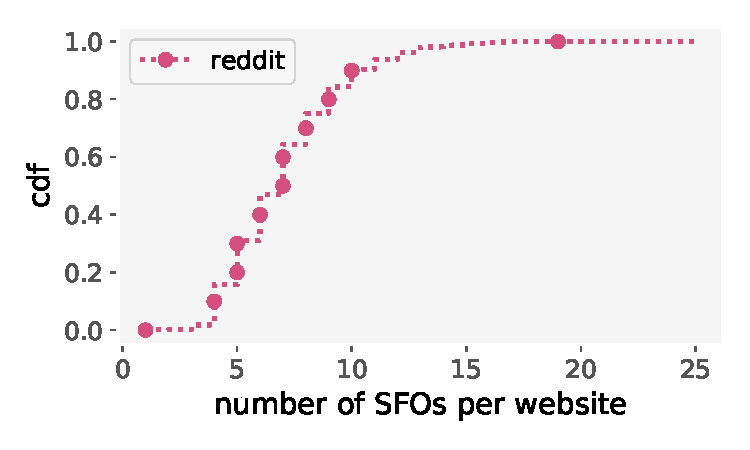
\includegraphics[width=\columnwidth]{../exp/plot/img/sfo-dist}
	\caption{%
		SFO distribution derived from the most frequently viewed reddit pages as
		of December 4, 2019.
	}
	\label{fig:sfo-dist}
\end{figure}

TODO: other overhead based on Mani et al (1--2 paragraphs)

\subsection{Flooding} \label{sec:flooding}

%As described in Section~\ref{sec:adversary}, an adversary might attempt to
%prevent an offending SFO from being sent to auditors by flooding
%one or all CTRs with SFOs. Abstractly, this could have two possible
%effects. If CTRs have a limited cache, which, once full, will not
%accept new SFOs, then the adversary can block the offending SFO
%from ever being held by any CTR by attempting to fill all
%CTR caches. If, however, a CTR might drop some cached SFOs
%so as to be able to cache some or all newly received SFOs, then
%the adversary can try to flush the cache of any CTR that might
%hold the offending SFO by flooding that CTR with new SFOs.
%
%A flooding attack could be directed at specific CTRs
%known or suspected of holding or being the intended recipient of
%an offending SFO\@. Our design, however, limits the ability of
%an adversary to know in advance the CTR to which a client will
%submit an offending SFO, or to know which CTR is holding
%an offending SFO until the CTR sends it to a log for auditing.
%And, at that point, there is no longer any point in flushing
%or blocking the CTR's cache.
%
%To have sufficient chance of succeeding, flooding attacks must thus be
%conducted against all CTRs in the network. To block, this would need to
%be sustained in anticipation of an offending SFO being received by
%a client or spun up quickly enough after a connection on which an
%offending SFO will be sent is initiated to fill all caches within
%seconds. Either would be highly visible and would require a
%DoS of Tor network resources that exceeds our threat model.\\
%***Need to justify that.***
%
%A flushing attack on all CTRs in the network has different time and
%knowledge parameters. The adversary need not flush CTRs before an
%offending SFO is sent. Indeed, that would be pointless. Once sent,
%however, the adversary must sustain a flooding attack so that the
%probability that the offending SFO is in any cache at the time of
%audit is very low. This gives the adversary effectively an interval
%of at least MMD to flush all CTR caches.
%
%To counter flushing, a CTR might adopt a combined strategy of caching
%some SFOs with a fixed or parameterized probability and dropping some
%SFOs from the cache with a separate fixed or parameterized
%probability. To simplify both design and analysis, our CTRs accept all
%inbound SFOs. Even if this exceeds the capacity of the cache, we
%assume the adversary is not able to exceed the combined capacity of
%the cache and inbound buffer. All cached and recently received SFOs
%are thus pooled together when considering which to drop. 
%
%By submitting an SFO for auditing at the earliest opportunity a CTR
%minimizes the risk of it being flushed and the load on its cache. On
%the other hand, by expanding the range of the random delay a CTR adds
%to MMD before auditing we expand the uncertainty of the adversary
%about whether or not the SFO might still be submitted, thus requiring
%him to both spend more resources and increase the risk of exposure by
%sustaining the flooding attack for a longer period.
%
%Overhead of a flushing attack for the adversary could be significantly
%raised and probability of attack success significantly diminished by
%following a strategy used by some types of mix in anonymous
%communication: make probabilistic the selection of individual SFOs
%amongst both the cached and newly received SFOs to be dropped as
%capacity of the cache is exceeded~\cite{trickle02}.
%
%
%Parameters:
%
%total CTR SFOs: those in the cache plus those in the inbound buffer\\
%CTR cache size\\
%randomized delay, uniform or decaying distribution?\\
%
%dropping strategies:
%
%uniform = total/cache-size\\
%MMD parameterized: Drop SFOs < MMD with one (lower) distribution,
%SFOs $\geq$ MMD with another (higher)\\
%Dynamic MMD parameterized: Drop only SFOs past MMD + constant until
%SFOs not yet to MMD exceeds cache size (following a Poisson or
%binomial distribution) . If only SFOs not yet to MMD are in the cache,
%then drop SFOs with a distribution that makes it more likely
%to drop a newer SFO from the cache until there are again some
%above MMD + constant.
%
%Advantage of the latter, is that it requires more resources for
%preventing an SFO from even making it to MMD. And by having randomized
%delays that follow, e.g., a Poisson or binomial distribution,
%the expected time an SFO must be cached is diminished and the
%chance of auditing before a flush is increased, even if
%the adversary optimizes its flooding strategy.

\subsection{Privacy}
At least mention privacy leaks to auditor. For example, related to CT logs
uptime. Caching of already resolved SFOs at CTRs reduce leak to CT logs and
auditors.

Push popular SFO hashes via TB

Tab-based caching (maybe not @privacy though)

\subsection{Design}

\subsubsection{CTR}
A CTR should be stable both to permit long-lived circuits to the CT logs and
to increase the likelihood of them staying online.

The criteria of being a middle relay, as opposed to an exit relay, follows
mainly from resource utilization considerations.  It is also about not making
exit relays ``more attractive targets'' due to also storing SFOs.

Note that we have a similar dilemma of disk avoidance in regular browsers too
(?), i.e., private mode

\subsubsection{Extension: Signal to CTRs}
On suspicion of network-wide attack, network health / auditors / DAs could
signal to CTRs through consensus flag to persist buffer of SFOs to disk for
later auditing to prevent loss on flooding or downtime. The reason for doing
this is that it shifts the potential \emph{impact} of detection (see
Section~\ref{sec:risk:impact}) from minor to potentially signfiicant or
catastrophic for the attacker.

There are huge privacy implications here, since the auditor gets a snapshot of
the current state of visited websites over Tor. At the very least, CTRs should
persist data in encrypted form (under provided public key in consensus), such as
not able to decrypt on its own to reduce risk of legal pressure on CTR
operators.

\subsubsection{CT Logs} \label{sec:discussion:logs}
Current landscape, log independence, accepted roots~\cite{ct-root-landscape}

(Non)available software.

\subsubsection{Incremental Deployment}
If $\texttt{ct-submit-pr} \gets 0$ and $\texttt{ct-max-sfo-bytes} \gets
\inf$, our design collapses into phase~1 and implies an SCT-centric CT policy
as used by Chrome/Safari.  Mb appeal for FF.

Base design can be put into practice without changing the log landscape or
requiering auditors that run reliable software (which doesn not exist right
now).

Ext:log appealing to make CT logs accountable

Ext:auditor also appleaing due to ecosystem value

Alternatively, goes in conclusion + impactful tor research
